\section{The Standard Model}
The Standard Model of particle physics (SM) describes all known particles and their non-gravitational interactions. Developed and experimentally verified over the past six decades, the SM posits the existence of twelve spin-$\frac{1}{2}$ particles, the fermions, that make up all observed matter; twelve spin-1 particles, the gauge bosons, that communicate the electromagnetic, weak, and strong forces; and one fundamental scalar, the Higgs boson, which breaks electroweak symmetry, giving mass to the gauge bosons and fermions.

The fermions and gauge bosons can be classified according to the forces with which they interact. The fermions are divided into six quarks, which carry color and interact via the strong force, and six leptons, which do not. Furthermore, all six quarks and three of the leptons carry electric charge and interact electromagnetically. The charged leptons include the electron, muon, and tau, and the neutral leptons are called neutrinos. All fermions interact via the weak force. The gauge bosons include the photon, which communicates the electromagnetic force; the \PWp, \PWm, and \cPZ\ bosons, which communicate the weak force; and eight gluons that communicate the strong force. Of these, only the \PWp\ and \PWm\ bosons are electrically charged and only the gluons carry color charge. Finally, the fermions are grouped into three generations, each with two quarks, one charged leptons, and one neutral lepton. Figure~\ref{sm_particles} diagrams the grouping of the SM particles and lists some of their properties.

\begin{figure}
\centering
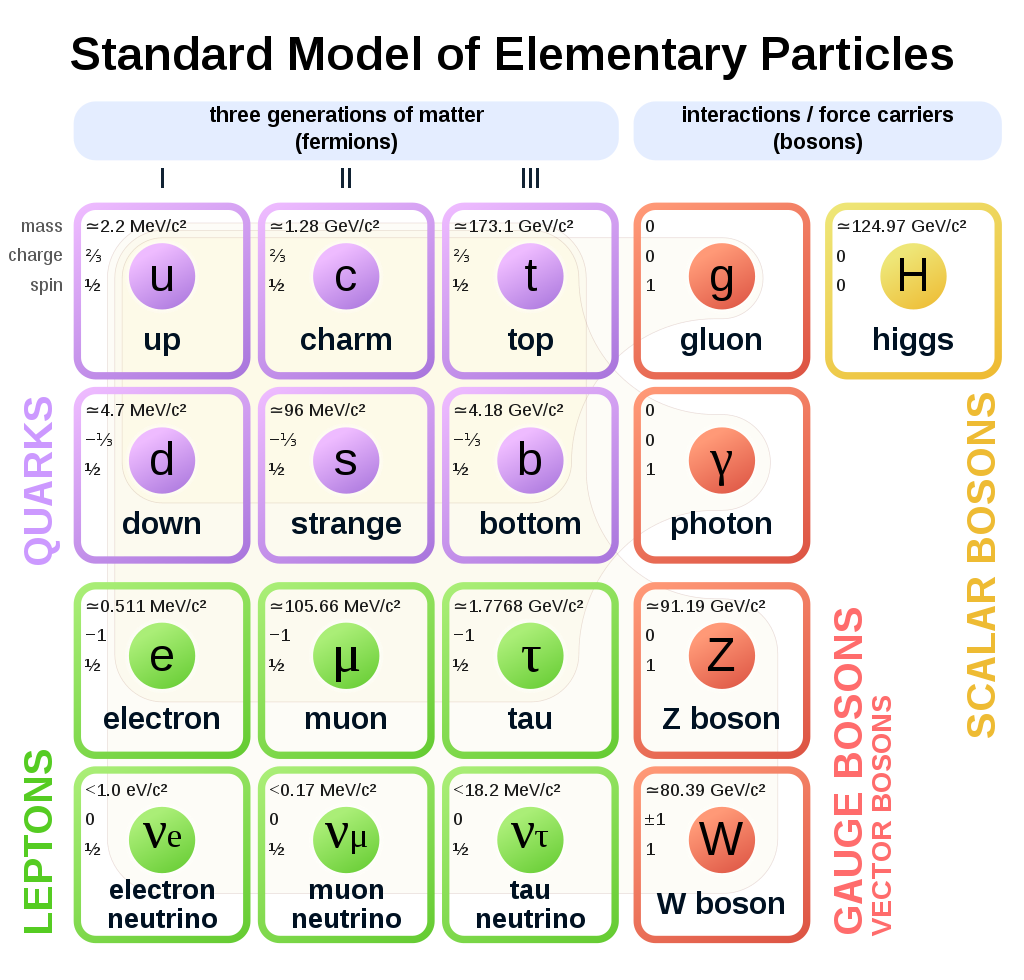
\includegraphics[scale=0.4]{figures/intro/sm_particles.png}
\caption{The Standard Model particle content.}
\label{sm_particles}
\end{figure}

In the SM, the interactions between particles are governed by two theories: quantum chromodynamics, which describes the strong force, and the electroweak theory, which describes the electromagnetic and weak forces. The following sections provide a brief overview of these theories.

\subsection{Quantum chromodynamics}
Quantum chromodynamics (QCD) describes the strong interactions between \linebreak[4]quarks and gluons and is based on the \suthreec\ symmetry group, where the subscript $\mathrm{c}$ refers to color charge. In QCD, all quarks and gluons carry color charge, which allows interactions between two quarks of the same generation and a gluon, three gluons, or four gluons. QCD is responsible for the formation of all hadrons (such as protons and neutrons), and leads to two unique phenomena: confinement and asymptotic freedom~\cite{gross_wilczek_73, qcd_73}.

Confinement refers to the experimental fact that an isolated particle with color charge has never been directly observed. Composite particles composed of quarks and gluons are always neutral under color, and attempts to separate the constituent particles will only produce new hadrons. This phenomenon is the result of the unique running of the strong coupling constant, which increases with decreasing energy (and therefore increasing distance).

Asymptotic freedom is the other side of the coin: if the strong coupling constant decreases as the interaction energy increases, then the strong interaction becomes more and more feeble at high energies. In high energy interactions (such as those at the Large Hadron Collider), the strong coupling constant is in fact small enough to render the quarks nearly free. In this regime, perturbative calculations become possible.

\subsection{The electroweak theory}
The electroweak theory unifies the electromagnetic and weak interactions and is based on the \ewsymm\ symmetry group. It posits two new charges: weak isospin, which has three components $T_{1}$, $T_{2}$, and $T_{3}$, and hypercharge, $Y$. $T_{3}$ is $\pm\frac{1}{2}$ for all left-handed fermions and 0 otherwise, while $Y$ varies according to $Q=T_{3}+\frac{1}{2}Y$, where $Q$ is the familiar electric charge. Each generation of left-handed quarks or leptons forms an $\mathrm{SU}(2)$ doublet. The first generation doublets, for example, are:
\begin{equation}
    \binom{\nu_{e}}{e^{-}}_{L},\ \binom{u}{d}_{L}
\end{equation}
where, as in \sutwol, the $\mathrm{L}$ denotes left-handed chiral states. The three generators of \sutwol\ result in three massless spin-1 bosons: $\mathrm{W}^{1}$, $\mathrm{W}^{2}$, and $\mathrm{W}^{3}$, while \uoney\ gives rise to one massless spin-1 boson, $\mathrm{B}^{0}$. After electroweak symmetry is broken by the mechanism explained in the following subsection, the physical \PWpm\ bosons are identified as superpositions of $\mathrm{W}^{1}$ and $\mathrm{W}^{2}$ while the \cPZ\ boson and the photon are identified as superpositions of $\mathrm{W}^{3}$ and $\mathrm{B}^{0}$~\cite{weinberg_leptons}.

Terms in the electroweak Lagrangian involve either two left-handed fermions and a \PWpm\ or \cPZ\ boson, two electrically charged particles and a photon, or charge-conserving combinations of \PWpm\ bosons, \cPZ\ bosons, and photons that include three or four particles. Conspicuously missing, however, are mass terms for the electroweak gauge bosons or fermions.

\subsection{The Higgs mechanism}
As shown in Fig.~\ref{sm_particles}, the fermions and \PWpm\ and \cPZ\ bosons all have nonzero mass. Accounting for this fact within the context of the electroweak theory is difficult because explicit mass terms violate the gauge and chiral symmetry of \ewsymm. For example, a term such as
\begin{equation}
    \frac{1}{2}m_{A}^{2}A^{\mu}A_{\mu},
\end{equation}
which assigns mass $m_{A}$ to gauge boson $A$, becomes
\begin{equation}
    \frac{1}{2}m^{2}(A^{\mu}-\partial^{\mu}\alpha)(A_{\mu}-\partial_{\mu}\alpha) \neq \frac{1}{2}m^{2}A^{\mu}A_{\mu}
\end{equation}
under a \uoney\ gauge transformation, and a term such as
\begin{equation}
    m_{f}\overline{f}f = m_{f}(\overline{f}_{R}f_{L} + \overline{f}_{L}f_{R}),
\end{equation}
which assigns mass $m_{f}$ to fermion $f$, breaks chiral symmetry by coupling the right- and left-handed components of the fermion.

If the gauge and chiral symmetries of \smsymm\ truly are symmetries of nature and the fermions and \PWpm\ and \cPZ\ bosons truly have nonzero mass, then another mechanism must be at work. Spontaneous symmetry breaking, which occurs when the vacuum state does not exhibit all of the symmetries of the underlying theory. In such a situation, each spontaneously broken continuous symmetry gives rise to a massless scalar particle~\cite{goldstone_salam_weinberg}. In the case of spontaneously broken continuous \textit{gauge} symmetries, however, there exists a mechanism by which the massless bosons are removed and some of the gauge bosons associated with the generators of the symmetries acquire mass~\cite{englert, higgs, kibble}. In the SM, this mechanism, known as the Higgs mechanism, breaks electroweak symmetry, gives mass to the fermions and \PWpm\ and \cPZ\ bosons, and results in one massive scalar particle, the Higgs boson.

The Higgs mechanism adds the scalar doublet
\begin{equation}
    \Phi = \binom{\phi^{+}}{\phi^{0}},
\end{equation}
whose potential is given by
\begin{equation}
    V(\Phi^{\dagger}\Phi) = \mu^{2}\Phi^{\dagger}\Phi + \lambda(\Phi^{\dagger}\Phi)^{2},
\end{equation}
to the SM. If $\mu^{2}<0$ and $\lambda>0$, then $\Phi^{\dagger}\Phi = -\frac{\mu^{2}}{2\lambda}$ defines a circle of minima in the $\phi^{+}$--$\phi^{0}$ plane. Even though the potential remains invariant under \ewsymm, nature must spontaneously choose a vacuum state somewhere along this circle. Because the vacuum state does not respect \ewsymm, the symmetry is said to be spontaneously broken.

This procedure has three significant consequences. First, three of the four degrees of freedom originally associated with $\Phi$ are now associated with the longitudinal components of the \PWpm\ and \cPZ\ bosons, which causes them to acquire mass while the photon remains massless. Second, $\Phi$'s remaining degree of freedom adds a single massive scalar, the Higgs boson, to the theory. Third, the interaction between the fermions and the nonzero vacuum state of the scalar field produces fermion mass terms that obey chiral symmetry.

\subsection{Current status}
\label{sm_status}
The SM is remarkably successful. It describes all known particles and their non-gravitational interactions, and it has passed countless experimental tests over the last several decades. Figure~\ref{cms_sm_measurements} gives an idea of the scale of this success by comparing theoretical predictions of SM production cross sections with measurements performed by the CMS experiment: theory and experiment agree across 41 different SM processes at \num{7}, \num{8}, and \SI{13}{\TeV}. In 2012, the CMS and ATLAS experiments  independently discovered an approximately \SI{125}{\GeV} scalar particle with properties consistent with the SM Higgs boson~\cite{cms_higgs, atlas_higgs}. Further measurements in \num{7}, \num{8}, and \SI{13}{\TeV} proton-proton collisions at the Large Hadron Collider continue to agree with SM predictions of the Higgs boson properties~\cite{cms_higgs_summary, atlas_higgs_summary}. We finally have meaningful evidence as to the origin of electroweak symmetry breaking, and all current evidence indicates that the SM Higgs mechanism is indeed responsible.

\begin{figure}
\centering
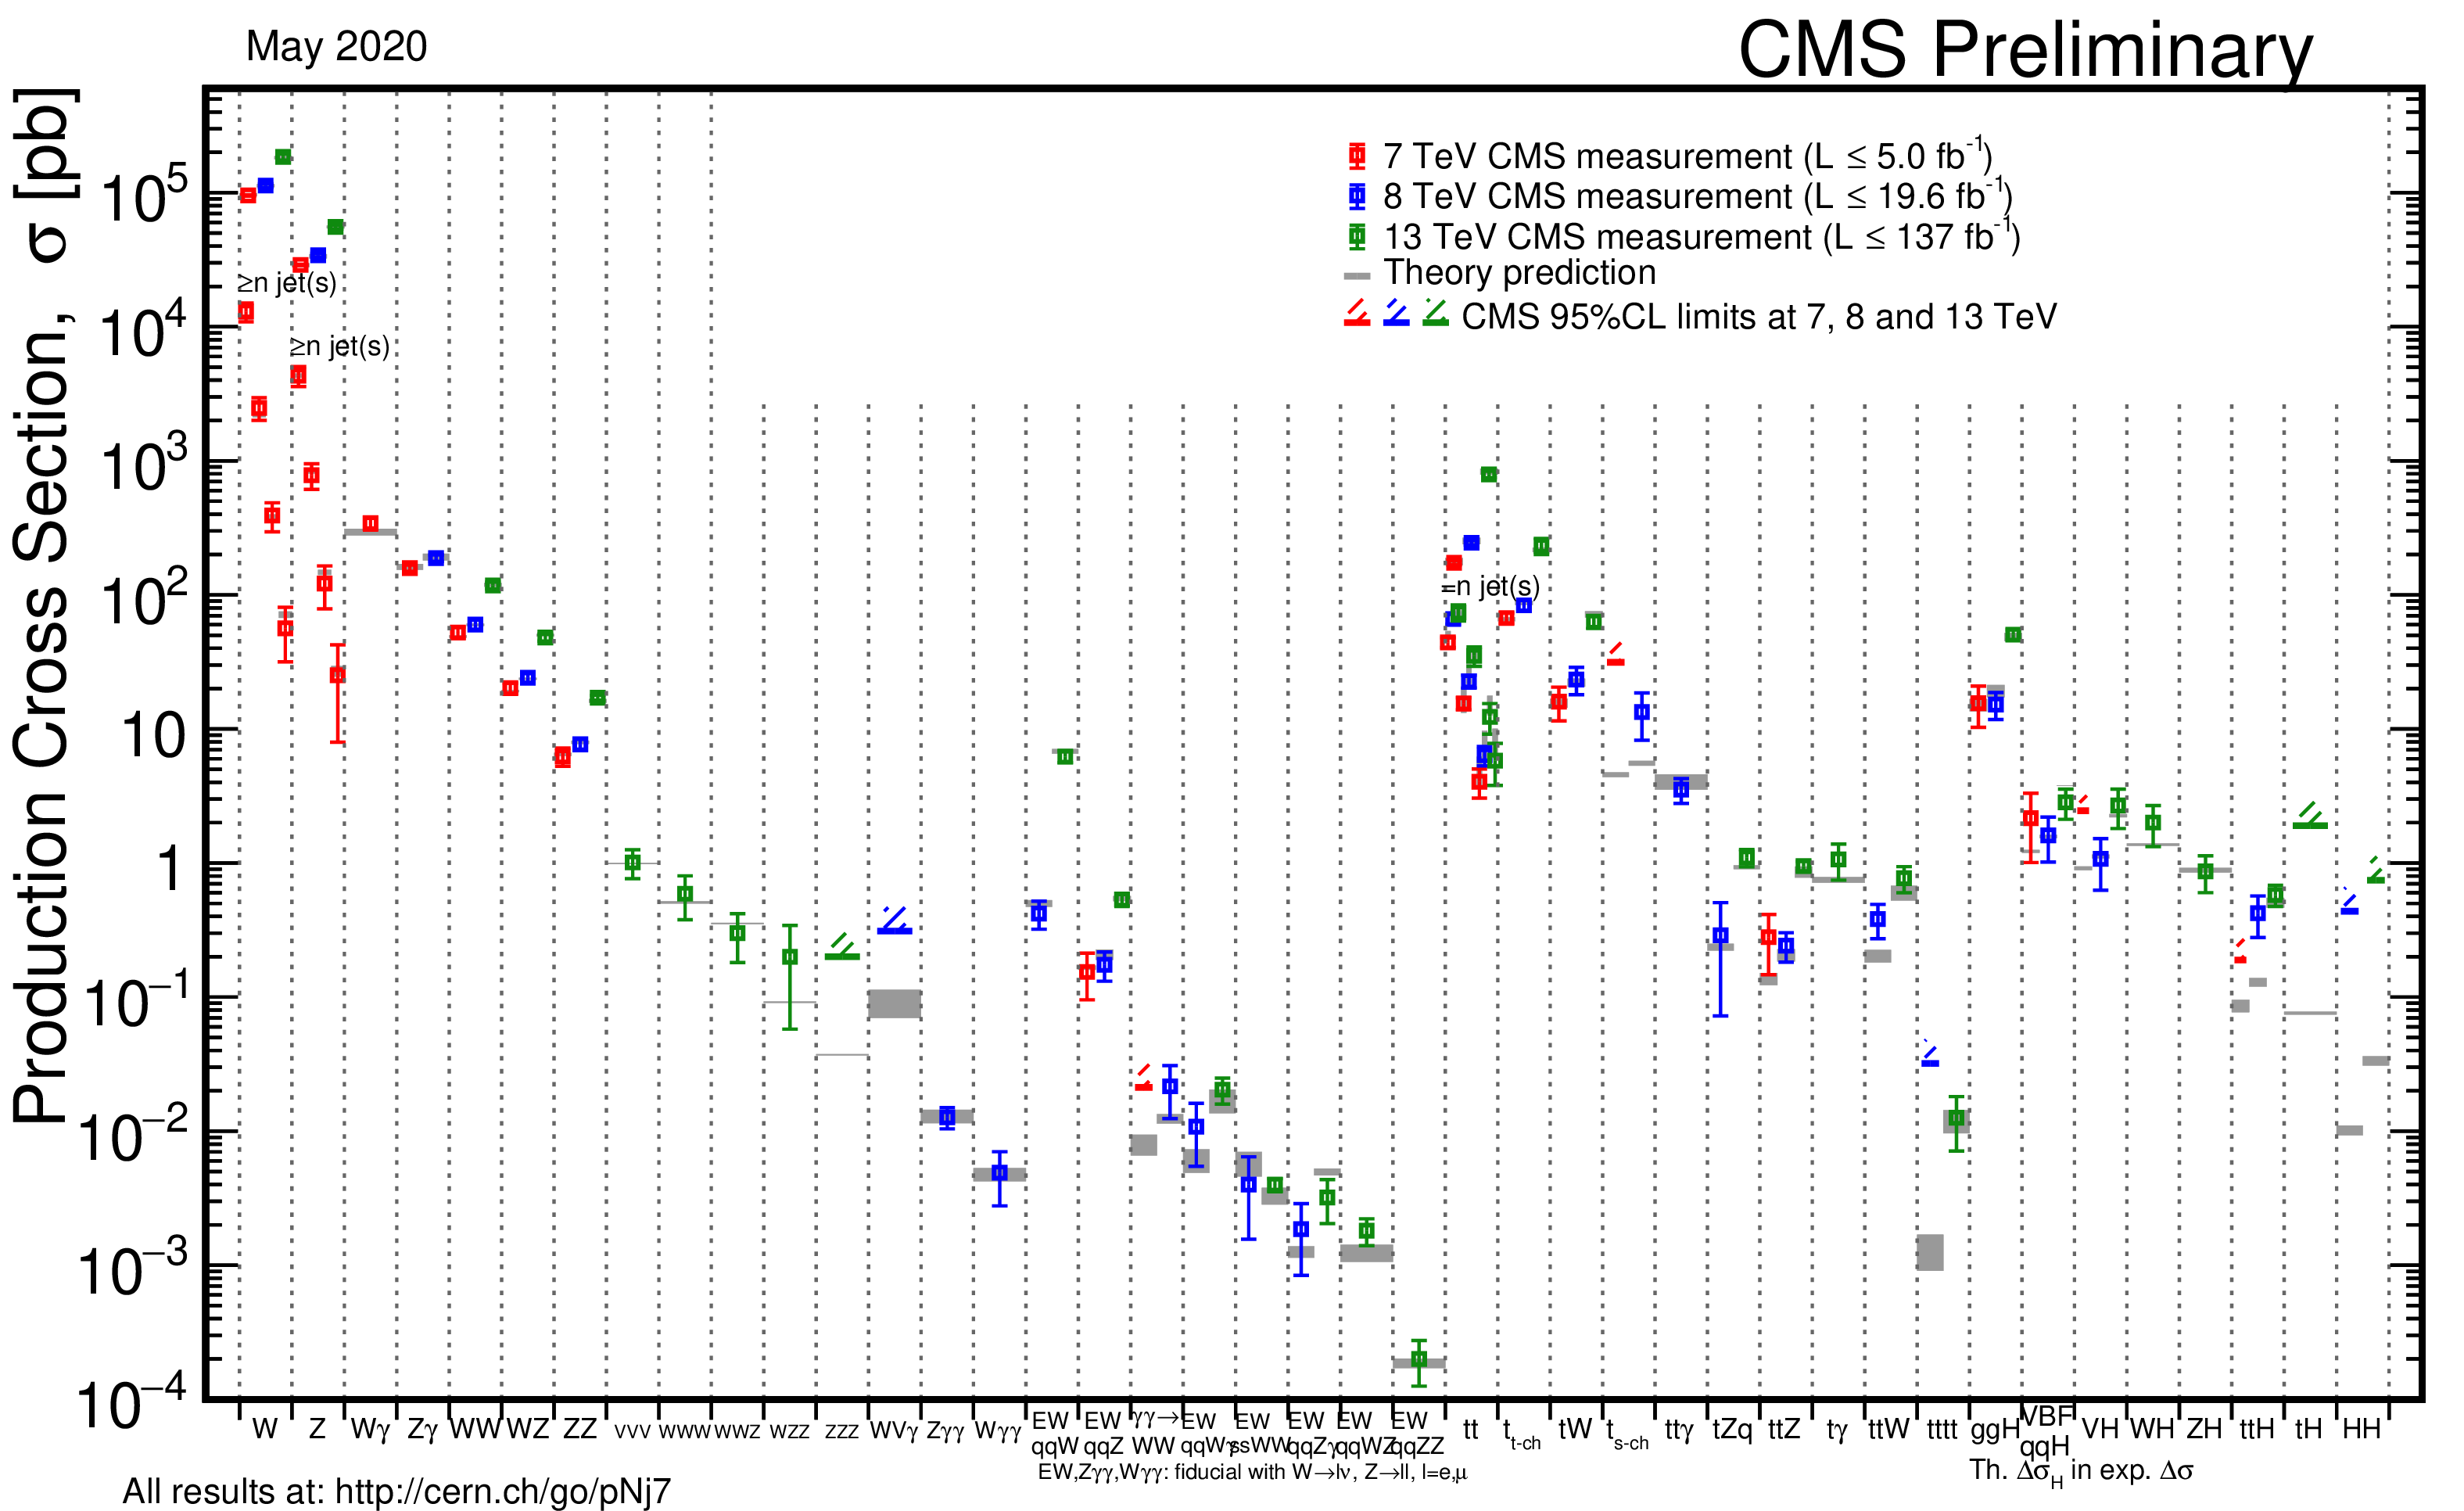
\includegraphics[width=\textwidth]{figures/intro/cms_sm_measurements.png}
\caption{Summary of Standard Model production cross section measurements from the CMS experiment \cite{cms_sm_public_results}.}
\label{cms_sm_measurements}
\end{figure}

Despite this remarkable success, the SM is not without problems. For one, it cannot be the whole story: it says nothing on the subjects of gravity, dark matter, or dark energy, which implies that it only describes about 5\% of the energy content of the universe~\cite{fukugita_2004} and that a more complete theory must take over at or below the energy scale where gravity becomes important ($M_{P}\approx\SI{e19}{\GeV}$)~\cite{giudice_naturalness_2008}. Furthermore, many aspects of the SM seem arbitrary and unmotivated. It offers no explanation, for example, for why three generations of fermions are necessary or why its many parameters take the values they do. It could be that these unmotivated values are simply experimental facts of nature without explanation, but the history of science implies that a deeper understanding is likely hiding beneath the surface. Finally, the observed value of the Higgs boson mass is not only unexplained, it is unnatural. This final issue, which is explained in the following paragraphs, is a powerful motivation to search for new physics at currently accessible energy scales.

\subsubsection{Naturalness}
The naturalness criterion states that an effective theory such as the SM must not be overly sensitive to the details of the underlying higher energy theory. Put another way, it requires that any dimensionless parameter much smaller than one must be protected by a custodial symmetry~\cite{thooft_naturalness}. Such a criterion may or may not be respected by nature, but history and simple probability are on its side.

The dimensionless parameter in question is the mass of the Higgs boson, which is quadratically sensitive to $\Lambda$, the energy scale at which a new theory takes over. All SM parameters are affected by interactions with virtual particles through loop diagrams such as those shown in Fig.~\ref{loop_diagrams}, but the Higgs boson mass is particularly sensitive. As a fundamental scalar, the Higgs boson lacks the chiral and gauge symmetries enjoyed by the fermions and gauge bosons. These symmetries, known as custodial symmetries, protect the fermion and gauge boson masses by guaranteeing that all corrections are proportional to the bare masses themselves. If the SM is indeed valid up to $M_{P}$, then the bare mass of the Higgs boson must be coincidentally equal and opposite to the sum of the terms that correct it to approximately one part in \num{e32}~\cite{giudice_naturalness_2008}. Such miraculous fine tuning is technically possible, but it could also be strong evidence that a deeper physical mechanism is at work.

\begin{figure}[hbtp]
\centering
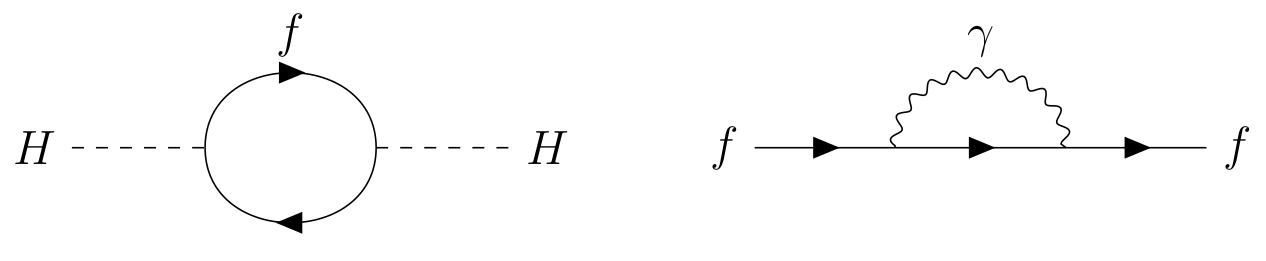
\includegraphics[scale=0.3]{figures/intro/loop_diagrams.png}
\caption{The Higgs boson mass corrected by a fermion loop (left) and a fermion mass corrected by photon loop (right).}
\label{loop_diagrams}
\end{figure}

\fxnote{make sure I don't refer to the Higgs mass when I really mean the square of the Higgs mass}
\fxnote{would be nice to add a paragraph arguing for physics at the weak scale}

\pagebreak